%%%%%%%%%%%%%%%%%%%%%%%%%%%%%%%%%%%%%%%
% Wenneker Resume/CV
% LaTeX Template
% Version 1.1 (19/6/2016)
%
% This template has been downloaded from:
% http://www.LaTeXTemplates.com
%
% Original author:
% Frits Wenneker (http://www.howtotex.com) with extensive modifications by 
% Vel (vel@LaTeXTemplates.com)
%
% License:
% CC BY-NC-SA 3.0 (http://creativecommons.org/licenses/by-nc-sa/3.0/
%
%%%%%%%%%%%%%%%%%%%%%%%%%%%%%%%%%%%%%%

%----------------------------------------------------------------------------------------
%	PACKAGES AND OTHER DOCUMENT CONFIGURATIONS
%----------------------------------------------------------------------------------------

\documentclass[a4paper,12pt]{memoir} % Font and paper size

%%%%%%%%%%%%%%%%%%%%%%%%%%%%%%%%%%%%%%%%%
% Wenneker Resume/CV
% Structure Specification File
% Version 1.1 (19/6/2016)
%
% This file has been downloaded from:
% http://www.LaTeXTemplates.com
%
% Original author:
% Frits Wenneker (http://www.howtotex.com) with extensive modifications by 
% Vel (vel@latextemplates.com)
%
% License:
% CC BY-NC-SA 3.0 (http://creativecommons.org/licenses/by-nc-sa/3.0/)
%
%%%%%%%%%%%%%%%%%%%%%%%%%%%%%%%%%%%%%%%%%

%----------------------------------------------------------------------------------------
%	PACKAGES AND OTHER DOCUMENT CONFIGURATIONS
%----------------------------------------------------------------------------------------

\usepackage[english,  russian]{babel}
\usepackage{XCharter} % Use the Bitstream Charter font
\usepackage[utf8]{inputenc} % Required for inputting international characters
\usepackage[T1]{fontenc} % Output font encoding for international characters

\usepackage[top=1cm,left=1cm,right=1cm,bottom=1cm]{geometry} % Modify margins

\usepackage{graphicx} % Required for figures

\usepackage{flowfram} % Required for the multi-column layout

\usepackage{url} % URLs

\usepackage[usenames,dvipsnames]{xcolor} % Required for custom colours

\usepackage{tikz} % Required for the horizontal rule

\usepackage{enumitem} % Required for modifying lists
\setlist{noitemsep,nolistsep} % Remove spacing within and around lists

\setlength{\columnsep}{\baselineskip} % Set the spacing between columns

% Define the left frame (sidebar)
\newflowframe{0.21\textwidth}{\textheight}{0pt}{0pt}[left]
\newlength{\LeftMainSep}
\setlength{\LeftMainSep}{0.21\textwidth}
\addtolength{\LeftMainSep}{1\columnsep}
 
% Small static frame for the vertical line
\newstaticframe{1.5pt}{\textheight}{\LeftMainSep}{0pt}
 
% Content of the static frame with the vertical line
\begin{staticcontents}{1}
\hfill
\tikz{\draw[loosely dotted,color=RoyalBlue,line width=1.5pt,yshift=0](0,0) -- (0,\textheight);}
\hfill\mbox{}
\end{staticcontents}
 
% Define the right frame (main body)
\addtolength{\LeftMainSep}{1.5pt}
\addtolength{\LeftMainSep}{1\columnsep}
\newflowframe{0.69\textwidth}{\textheight}{\LeftMainSep}{0pt}[main01]

\pagestyle{empty} % Disable all page numbering

\setlength{\parindent}{0pt} % Stop paragraph indentation

%----------------------------------------------------------------------------------------
%	NEW COMMANDS
%----------------------------------------------------------------------------------------

\newcommand{\userinformation}[1]{\renewcommand{\userinformation}{#1}} % Define a new command for the CV user's information that goes into the left column

\newcommand{\cvheading}[1]{{\Huge\bfseries\color{RoyalBlue} #1} \par\vspace{.6\baselineskip}} % New command for the CV heading
\newcommand{\cvsubheading}[1]{{\Large\bfseries #1} \bigbreak} % New command for the CV subheading

\newcommand{\Sep}{\vspace{1em}} % New command for the spacing between headings
\newcommand{\SmallSep}{\vspace{0.5em}} % New command for the spacing within headings

\newcommand{\aboutme}[2]{ % New command for the about me section
\textbf{\color{RoyalBlue} #1}~~#2\par\Sep
}
	
\newcommand{\CVSection}[1]{ % New command for the headings within sections
{\Large\textbf{#1}}\par
\SmallSep % Used for spacing
}

\newcommand{\CVItem}[2]{ % New command for the item descriptions
\textbf{\color{RoyalBlue} #1}\par
#2
\SmallSep % Used for spacing
}

\newcommand{\bluebullet}{\textcolor{RoyalBlue}{$\circ$}~~} % New command for the blue bullets
 % Include the file specifying document layout and packages

%----------------------------------------------------------------------------------------
%	NAME AND CONTACT INFORMATION 
%----------------------------------------------------------------------------------------

\userinformation{ % Set the content that goes into the sidebar of each page
\begin{flushright}
% Comment out this figure block if you don't want a photo
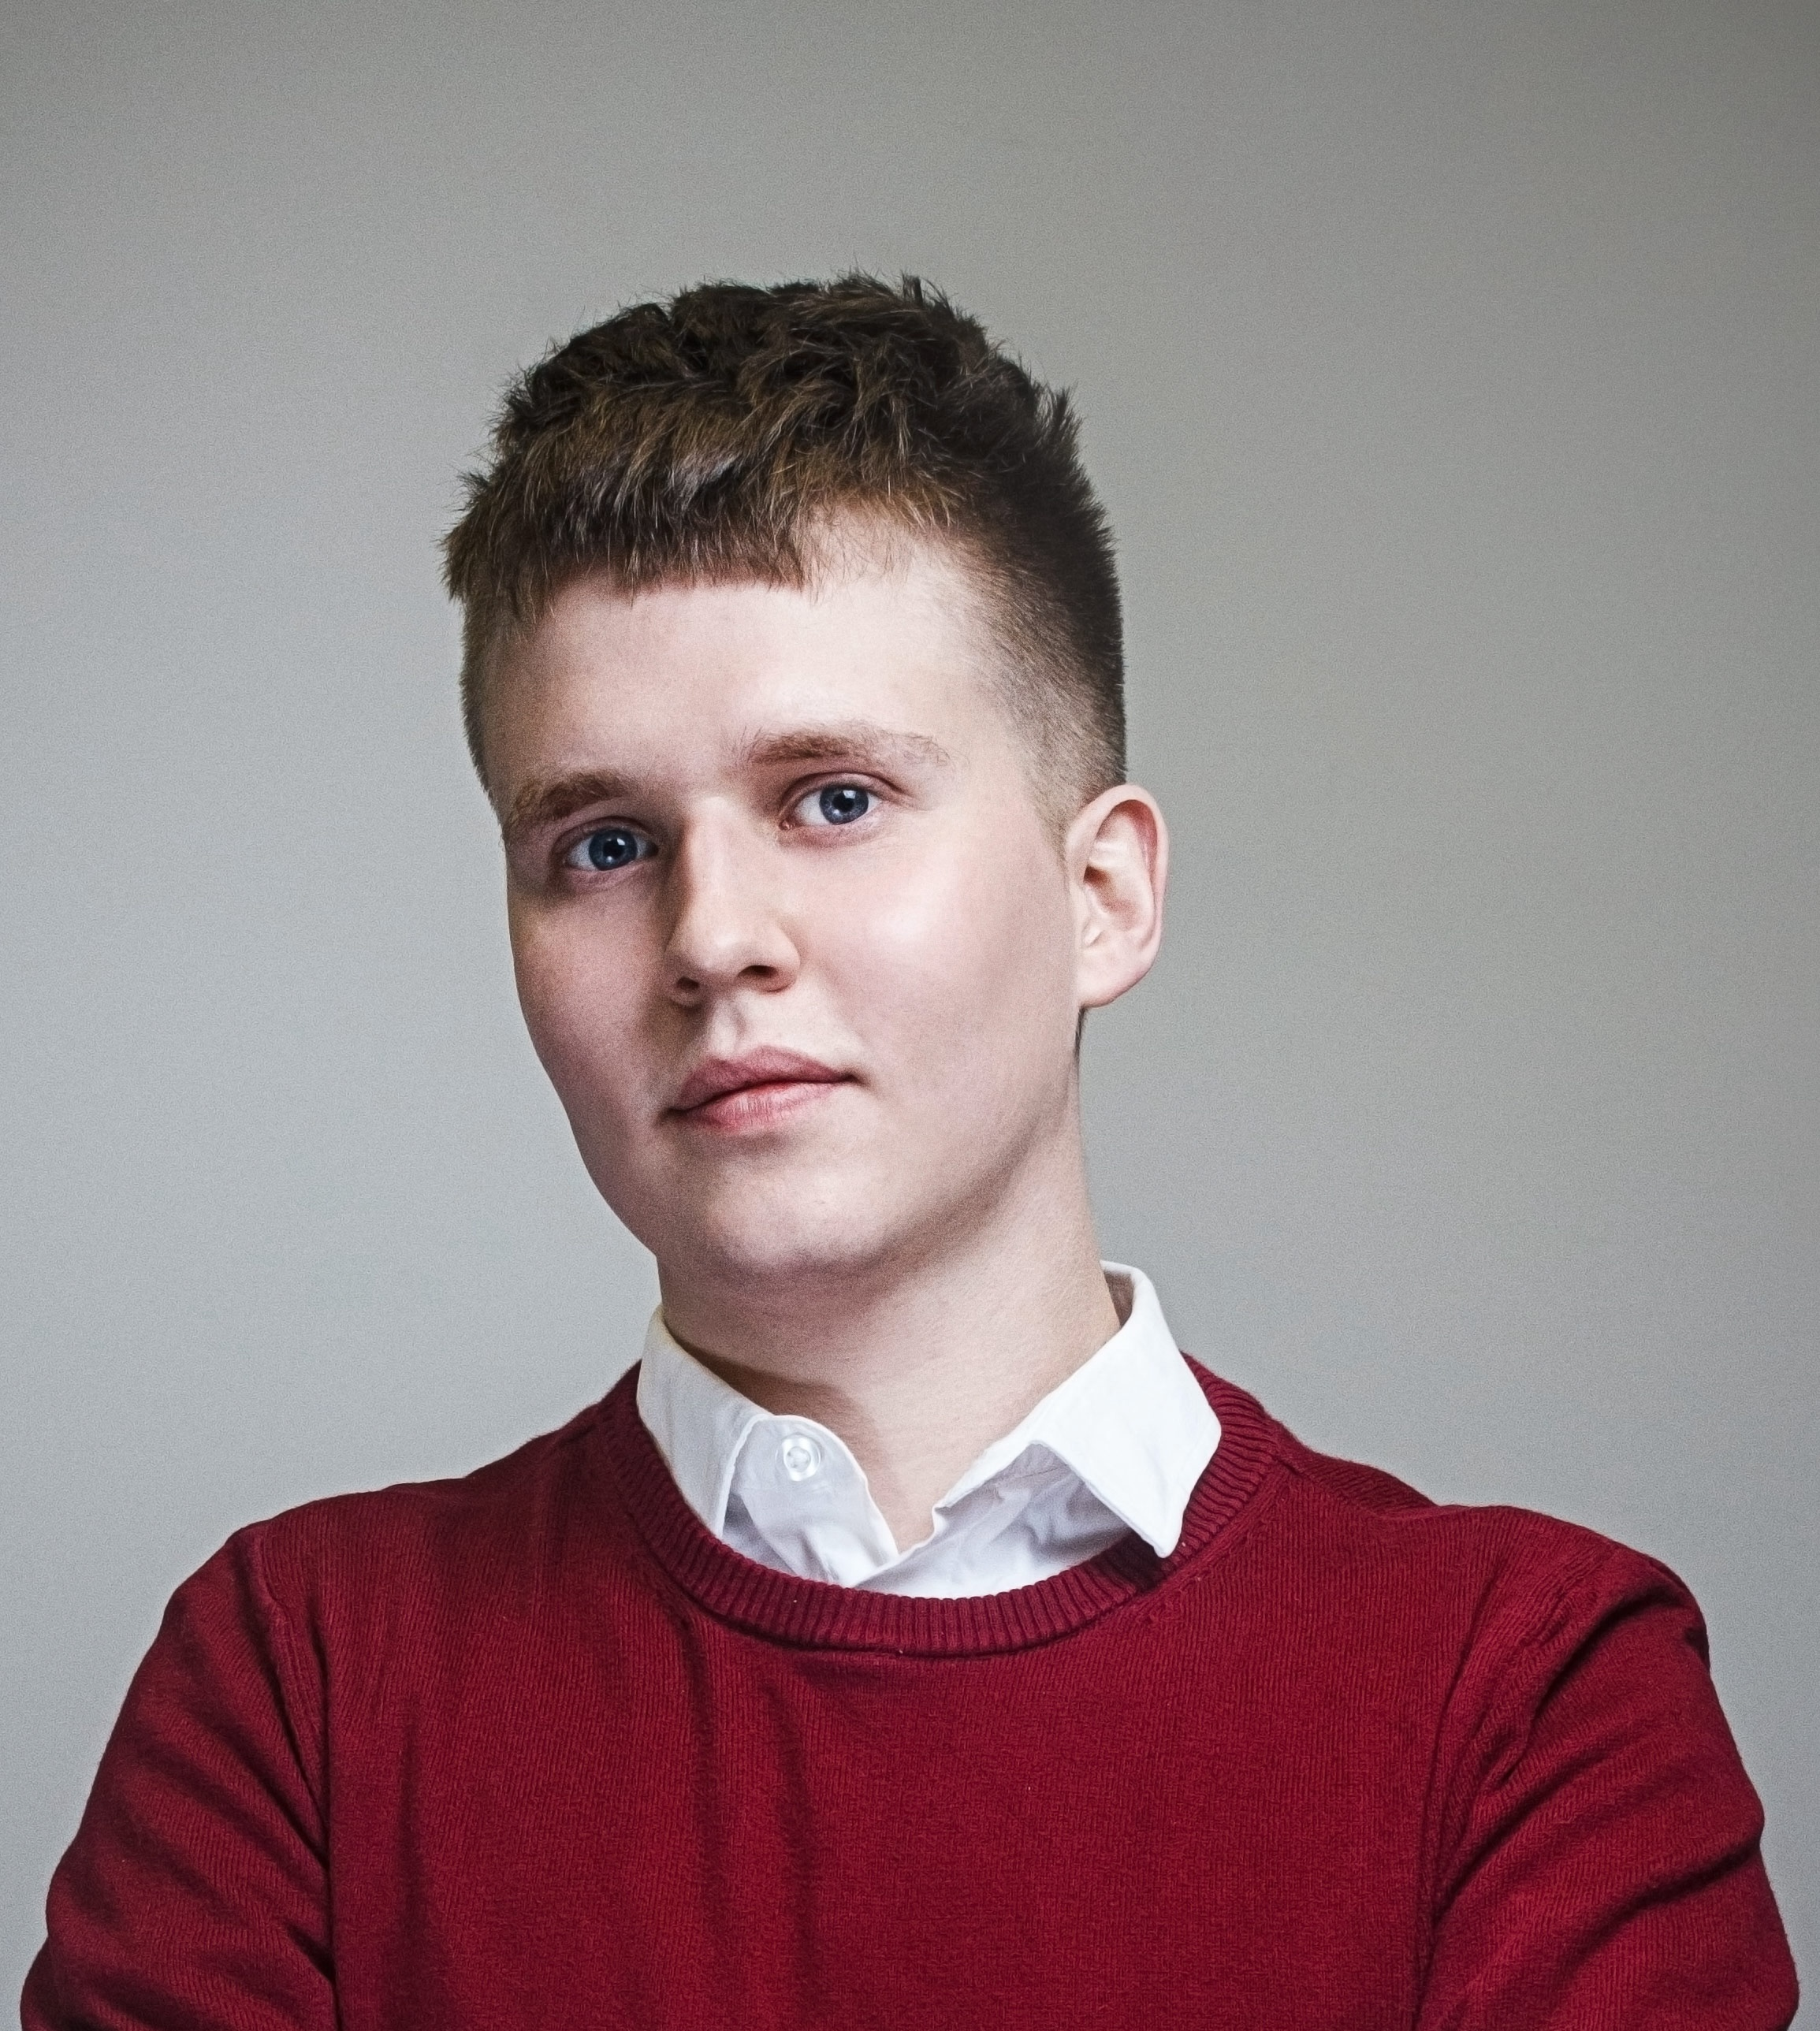
\includegraphics[width=1.0\columnwidth]{my_photo}\\[\baselineskip] % Your photo
\small % Smaller font size
\textbf{Alexander Piskotin} \\ % Your name
\href{mailto:aapiskotin.ge@gmail.com}{\url{aapiskotin.ge@gmail.com}} \\ % Your email address
+995 (595) 116-387 \\ % Your phone number
\href{https://t.me/gabgabgabgab}{\faTelegram}/
\href{https://wa.me/995595116387}{\faWhatsapp}/
\href{https://www.linkedin.com/in/aapiskotin/}{\faLinkedin}
\\ % tg/wa/li

\Sep % Some whitespace
\textbf{Current Location} \\
Tbilisi, Georgia \\
\Sep % Some whitespace
\textbf{Languages} \\
Russian - C2[\textit{native}] \\
English - B2[
	\href{https://drive.google.com/file/d/1WWuvrctOhVMc2_1UgOc5NAVF9zPU3J3c/view?usp=sharing}
		{\textit{Pipplet}}
] \\

\vfill % Whitespace under this block to push it up under the photo
\end{flushright}
}

%----------------------------------------------------------------------------------------

\begin{document}

\userinformation % Print your information in the left column

\framebreak % End of the first column

%----------------------------------------------------------------------------------------
%	HEADING
%----------------------------------------------------------------------------------------

\cvheading{Alexander Piskotin} % Large heading - your name

\cvsubheading{Machine Learning Engineer} % Subheading - your occupation/specialization

%----------------------------------------------------------------------------------------
%	ABOUT ME
%----------------------------------------------------------------------------------------

\aboutme{About Me}{
	Experienced Machine Learning Engineer adept at developing and implementing advanced
	algorithms that drive process optimization, user engagement, and profitability across AdTech,
	digitial marketing, finance, social platforms and e-commerce.
	Focused on crafting innovative, data-driven engineering solutions that
	significantly enhance business operations and efficiency.
}

%----------------------------------------------------------------------------------------
%	EXPERIENCE
%----------------------------------------------------------------------------------------

\CVSection{Experience}

%------------------------------------------------

\CVItem{Apr 2022 -- Present, \textit{ML Engineer},\\ \href{https://socialdiscoverygroup.com/}{Social Discovery Group}[\textit{Dating/Entertainment Platforms}]}{
\begin{itemize}
	\item DSP (\textit{Demand Side Platform})
	\begin{itemize}
		\item Spearheaded the development of bid optimization algorithms for a DSP in AdTech
		\item Successfully reducing CPC(\textit{Cost per Click}) by 25\% and CPM(\textit{Cost per Mile}) by 75\% in remarketing campaigns through a series of experiments
		\item Introduced results at webinar: \href{https://www.youtube.com/watch?v=UR7ba3vMiN4}{\textit{"In-house DSP. Optimal Bidding Problem"}}
	\end{itemize}
	\item Virtual Gifts Ranking
	\begin{itemize}
		\item Led the development of a ranking algorithm for virtual gifts in chats
		\item Increased user engagement by 25\% and virtual gift spending per paying user by 18\%
	\end{itemize}
	\item DDA (\textit{Data-Driven Attribution})
	\begin{itemize}
		\item Engineered and deployed a novel marketing campaign performance measurement algorithm using a Recurrent Neural Network
		\item Achieved a 6\% increase in eROI(expected Return on Investment)
	\end{itemize}
	\item Machine Learning for Direct Marketing
	\begin{itemize}
		\item Developed a machine learning solution that optimized email campaign efficiency
		\item Reduced email volume by 50\% without compromising engagement (less than 5\% drop in clicks), thereby preserving core business metrics.
	\end{itemize}
	\item Landing Page Optimization
	\begin{itemize}
		\item Initiated a continuous testing framework for landing pages using a Multi-Armed Bandit algorithm
		\item Boosted conversion rates by 15\%.
	\end{itemize}
	\item Chat Copilot Implementation
	\begin{itemize}
		\item Contributed to the team that implemented an LLM-driven chat copilot
		\item Enhanced user interaction and operational efficiency. The project gained positive unit-economics since the first experiment iteration
	\end{itemize}
	\item LTV Prediction Models
	\begin{itemize}
		\item Created and deployed multiple LTV(\textit{LifeTime Value}) prediction models
		\item Increased marketing campaigns efficiency (up to +25\% in eROI per campaign)
			via usage as predictive conversions
	\end{itemize}
\end{itemize}
}

%------------------------------------------------

\CVItem{Feb 2024, \textit{Hackathon Jury/Expert (Volunteering)}, \href{https://www.zavodit.ru/ru/calendar/event/46}{ML TalentMatch}, \href{https://ac-vo.ru/}{AC-VO}}{
\begin{itemize}
	\item Evaluated and provided feedback on the projects of the participants
	\item Assessed the technical and business aspects of the ML solutions
\end{itemize}
}
\Sep % Extra whitespace after the end of a major section

%------------------------------------------------

%----------------------------------------------------------------------------------------
%	NEW PAGE DELIMITER
%	Place this block wherever you would like the content of your CV to go onto the next page
%----------------------------------------------------------------------------------------

\clearpage % Start a new page

\userinformation % Print your information in the left column

\framebreak % End of the first column

%------------------------------------------------

\CVItem{Dec 2020 -- Apr 2022, \textit{ML Engineer}, \href{https://bki-okb.ru/}{United Credit Bureau}}{
\begin{itemize}
	\item Real-Time Scoring System
	\begin{itemize}
		\item Engineered and maintained a real-time scoring system that includes a feature store and models service.
			My work encompassed integrating models, designing an additional abstraction layer for easier model integration by the data science team,
			implementing a model testing approach, and developing middleware for real-time ML monitoring.
		\item Significantly reduced time-to-market for new models and features, and improved the overall quality of the scoring system
	\end{itemize}
	\item Captcha Solver Algorithm
	\begin{itemize}
		\item Led the development and enhancement of a Captcha solver algorithm that significantly increased data update frequency
		\item Improved the relevancy of the credit scoring data by providing
		more frequent updates, which results in increased accuracy of scoring models
	\end{itemize}
	\item Revenue/Profit Prediction Algorithm
	\begin{itemize}
		\item Created a predictive algorithm for businesses' revenue and profits estimation
		\item Integrated as a B2B service providing targeting data for financial
			products advertisement
	\end{itemize}
	\item Income Prediction Model
	\begin{itemize}
		\item Developed and successfully integrated an individual's income prediction model based on credit history data
		\item Deployed as a profitable B2B solution.
	\end{itemize}
	\item Custom Credit Scoring Models
	\begin{itemize}
		\item Designed and developed bespoke credit scoring models for diverse B2B clients
		\item Passed all on-site validations and were integrated into clients’ credit scoring pipelines
	\end{itemize}
%	\item Machine Learning Utilities Package
%	\begin{itemize}
%		\item Contributed significantly to the development of an internal machine learning utilities package,
%			greatly reducing time-to-market for deploying new models and features
%	\end{itemize}
\end{itemize}
}

%------------------------------------------------

\CVItem{Oct 2019 -- Feb 2022, \textit{Research Engineer (Apprenticeship)}, \href{https://ipmnet.ru/}{Ishlinsky Institute for Problems in Mechanics RAS}}{
\begin{itemize}
	\item Automation Tools Development
	\begin{itemize}
		\item Developed and implemented a suite of automation tools for data collection
			in experimental environments
		\item Significantly increased the number of samples gathered per a period of time,
			which allowed collecting datasets for statistical analysis
	\end{itemize}
	\item Experimental Data Analysis in Physics of Fluids
	\begin{itemize}
		\item Designed and implemented various experimental setups on unique equipment stand.
			Collected and analyzed large sets of hydrophone data.
		\item Resulted in a publication and a conference presentation
	\end{itemize}
\end{itemize}
}

\CVItem{Jul 2019 -- Nov 2020, \textit{Junior Data Scientist}, \href{https://www.utkonos.ru/}{Utkonos}[\textit{Online Grocery Store}]}{
\begin{itemize}
	\item Uplift Modeling for Direct-Marketing
	\begin{itemize}
		\item Led the development of an uplift model for promocodes, strategically targeting customers whose engagement would yield a positive margin
		\item This approach increased Average Revenue Per User (ARPU) by 2.8\% and improved margin per user by 3.2\%
	\end{itemize}
%	\item Customer Segmentation Insights
%	\begin{itemize}
%		\item Provided the direct marketing team with crucial insights by employing
%			customer clustering based on RFM (Recency, Frequency, Monetary value) and
%			basket analysis features, enhancing targeted marketing strategies
%	\end{itemize}
%	\item Recommender System Baseline
%	\begin{itemize}
%		\item Developed a baseline solution for a recommender system, setting the stage for personalized customer experiences and increased engagement
%	\end{itemize}
	\item Warehouse Digital Twin Development
	\begin{itemize}
		\item Contributed to the creation of a digital twin model for the warehouse, enabling robust hypothesis testing and operational optimization
	\end{itemize}
%	\item A/B Testing for Data Science
%	\begin{itemize}
%		\item Assisted in the design and analysis of A/B tests for the data science team,
%			contributing to the validation and refinement of models and strategies through empirical data analysis
%	\end{itemize}
\end{itemize}
}

%----------------------------------------------------------------------------------------
%	NEW PAGE DELIMITER
%	Place this block wherever you would like the content of your CV to go onto the next page
%----------------------------------------------------------------------------------------

\clearpage % Start a new page

\userinformation % Print your information in the left column

\framebreak % End of the first column

%------------------------------------------------

\CVItem{Jul 2019 -- Nov 2020, \textit{Junior Data Scientist}, \href{https://www.utkonos.ru/}{Utkonos[\textit{Online Grocery Store}]}}{
\begin{itemize}
%	\item Uplift Modeling for Direct-Marketing
%	\begin{itemize}
%		\item Led the development of an uplift model for promocodes, strategically targeting customers whose engagement would yield a positive margin
%		\item This approach increased Average Revenue Per User (ARPU) by 2.8\% and improved margin per user by 3.2\%
%	\end{itemize}
	\item Customer Segmentation Insights
	\begin{itemize}
		\item Provided the direct marketing team with crucial insights by employing
			customer clustering based on RFM (Recency, Frequency, Monetary value) and
			basket analysis features, enhancing targeted marketing strategies
	\end{itemize}
%	\item Recommender System Baseline
%	\begin{itemize}
%		\item Developed a baseline solution for a recommender system, setting the stage for personalized customer experiences and increased engagement
%	\end{itemize}
%	\item Warehouse Digital Twin Development
%	\begin{itemize}
%		\item Contributed to the creation of a digital twin model for the warehouse, enabling robust hypothesis testing and operational optimization
%	\end{itemize}
	\item A/B Testing for Data Science
	\begin{itemize}
		\item Assisted in the design and analysis of A/B tests for the data science team,
			contributing to the validation and refinement of models and strategies through empirical data analysis
	\end{itemize}
\end{itemize}
}

%------------------------------------------------

\Sep % Extra whitespace after the end of a major section

%----------------------------------------------------------------------------------------
%	EDUCATION
%----------------------------------------------------------------------------------------

\CVSection{Education}

%------------------------------------------------

\CVItem
	{
		2016 -- 2022,
		National Research Nuclear University MEPhI (Moscow Engineering Physics Institute)
	}
	{
		\textbf{(Adj.) GPA 3.565}, Specialist Qualification,
		Electronics and automation of physical installations/Physicist engineer
	}

\CVItem{2023, karpov.Courses. \href{https://karpov.courses/ml-hard}{HARD ML}}
{
	\href{https://lab.karpov.courses/certificate/052af508-2d33-4b20-b8c2-21c826b4d40b/en/}{
		Modules: Uplift Modelling, Dynamic Pricing, Ranking and Matching,
		Advanced A/B Testing, ML-Services: Deployment
	}
}

\CVItem{2019, Mail.ru Group. \href{https://technoatom.vk.company/}{Technoatom}}{Applied Python: Machine Learning, Deep Learining}

%------------------------------------------------

\Sep % Extra whitespace after the end of a major section

%----------------------------------------------------------------------------------------
%	SKILLS
%----------------------------------------------------------------------------------------

\CVSection{Skills}

%------------------------------------------------

\CVItem{ML Applications}
{\begin{tabular}{p{0.2\textwidth} p{0.2\textwidth} p{0.2\textwidth}}
\bluebullet Uplift Modelling & \bluebullet Dynamic Pricing & \bluebullet Ranking\\
\bluebullet NLP & \bluebullet CV & \bluebullet RL\\
\bluebullet Forecasting & \bluebullet Credit Scoring & \bluebullet Predictive Models\\
\end{tabular}}

\CVItem{Productionalization}
{\begin{tabular}{p{0.2\textwidth} p{0.2\textwidth} p{0.2\textwidth}}
\bluebullet Feature Store & \bluebullet MLOps & \bluebullet ML Monitoring\\
\bluebullet ETL & \bluebullet  Feedback Loop & \bluebullet A/B Testing\\
\end{tabular}}

\CVItem{Tools}
{\begin{tabular}{p{0.2\textwidth} p{0.2\textwidth} p{0.2\textwidth}}
\bluebullet Python & \bluebullet SQL & \bluebullet AWS\\
\bluebullet Apache Airflow & \bluebullet Apache Spark & \bluebullet Hadoop\\
\bluebullet Kubernetes & \bluebullet Docker & \bluebullet Kafka\\
\end{tabular}}

%------------------------------------------------

\Sep % Extra whitespace after the end of a major section

%----------------------------------------------------------------------------------------
%	Publications
%----------------------------------------------------------------------------------------

\CVSection{Publications}

%------------------------------------------------

%\CVItem{
%	\href{https://drive.google.com/file/d/18ssY54vQuOrl3tguyuYBVDMOgzzkC7Zy/view?usp=sharing}
%	{Оптимизация Аппроксимирующего Полинома Передаточной Функции Гидрофона в Целях
%	Экстраполяции Градуировочной Характеристики в Область Высоких Частот}
%	(\textit{Optimization of the Approximating Polynomial of the Hydrophone Transfer Function for the Purpose of Extrapolation of the Calibration Characteristic to the High Frequency Region Using Bayesian Optimization Methods})
%}
%{Jan 2022, National Research Nuclear University MEPhI/Ishlinsky Institute for Problems in Mechanics RAS}

%------------------------------------------------

\CVItem{
	\href{https://www.youtube.com/watch?v=UR7ba3vMiN4}
	{In-house DSP. Optimal Bidding Problem}
}
{Feb 2023, Webinar "Algorithms of Love. Machine Learning in Social Discovery"{}, Social Discovery Group}

%---------------------------------------------

\CVItem{\href{http://www.reglament.net/bank/credit/2021_6/get_article.htm?id=7298}{Риск-факторы как фактор неэффективности кредитного конвейера} (\textit{Risk-Factors - the Factors of Ineffective Credit Pipeline})}
{Dec 2021, «Банковское кредитование» journal, Publishing House «Регламент»}

%------------------------------------------------

\CVItem{
	\href{http://www.spsl.nsc.ru/FullText/konfe/ВолныВихриX.pdf}
	{Регистрация капельных течений и сопутствующих звуковых пакетов}
	(\textit{Recording drip currents and accompanying sound packets})
}
{Dec 2019, Waves and vortices in complex media, Ishlinsky Institute for Problems in Mechanics RAS}

\Sep % Extra whitespace after the end of a major section

%----------------------------------------------------------------------------------------

\end{document}
